%!TEX root = ../main.tex

We implemented the procedures and optimizations in Section~\ref{sec:algorithm}-\ref{sec-opt-sol-gen} on top of OSTRICH, resulted to a string solver called $\ostrichrecl$. 
%
In this section, we evaluate the performance of $\ostrichrecl$ on three benchmark suites, that is, RegCoL, AutomatArk, and NestC. In the sequel, we first describe the three benchmark suites as well as the experiment setup. Then we present the experiment results. We evaluate the performance and correctness of our solver against the state-of-the-art string constraint solvers, including CVC5 \cite{cvc5}, Z3seq \cite{z3seq}, Z3str3 \cite{Z3-str3}, Z3str3RE \cite{BD+23}, and OSTRICH \cite{CHL+19}. We also compare $\ostrichrecl$ with several variants of itself, to evaluate the effectiveness of the technical choices and optimizations in Section~\ref{sec:algorithm}-\ref{sec-opt-sol-gen}.

% We do experiments to compare the performance of $\ostrichrecl$ with the state-of-the-art string solvers. Moreover, in order to know whether $\ostrichrecl$ is good at solving string constraints with large counting and length, we extract \denghang{todo} instances with large bounds out of , and compare the performance of $\ostrichrecl$ with the other solvers on these instances. Finally, we empirically justify the technical choices made in the decision procedure of Section~\ref{subsec:cefadec} by comparing $\ostrichrecl$ with the following two variants of $\ostrichrecl$: $\ostrichrecl_{\rm - ASR}$ and $\ostrichrecl_{\rm NUXMV}$, where $\ostrichrecl_{\rm - ASR}$ and $\ostrichrecl_{\rm NUXMV}$ are obtained from $\ostrichrecl$ by removing the automata size-reduction technique (i.e. Step 2 in Section~\ref{subsec:cefadec}) and using the nuXmv model checker to solve the nonemptiness of $\cefadec$ respectively. 
 
%including the results for an overall evaluation as well as the results on the benchmark instances with large bounds. Moreover, we do experiments to show the effectiveness of the automata size-reduction technique (i.e. Step 2 in Section~\ref{sec:algorithm}) as well as compare $\ostrichrecl$ with the  nuXmv-based approach in \cite{atva2020}.  

%Then we present experiment results of the large-counting part and evaluate the simplification techniques. The goal of our experiments is to answer the following questions:
%\begin{itemize}
%  \item [Q1:] Does the decision procedure perform well~(Sec \ref{subsec:overall_eval}), especially when the counting bounds are large?~(Sec \ref{subsec:large_bounds_eval})
%  \item [Q2:] Are the size-reduction techniques practical?~(Sec \ref{subsec:size_reduction_eval})
%  \item [Q3:] How effective is the algorithm for solving the nonemptiness problem compared to the case that uses the nuXmv model checker~\cite{atva2020}?~(Sec \ref{subsec:size_reduction_eval})
%\end{itemize}



\subsection{Benchmark suites and the experiment setup}\label{sec:bench}

Our experiments utilize three benchmark suites, namely, \emph{RegCoL}, \emph{AutomatArk}, and \emph{NestC}. 
%Other benchmark suites are not utilized because they contain no counting operators. 
There are 49,843 instances in total.
%, where 48,843 of them are collected from the real world and 1,000 of them are generated by the string fuzzing tool. 
All benchmark instances are in the SMTLIB2 format. In the sequel, we give more details of these three benchmark suites.

\medskip
\noindent
\emph{RegCoL benchmark suite.} There are 40,628 RECL instances in the RegCoL suite. These instances are generated by extracting regexes with counting operators from the open source regex library \cite{regex_lingua_franca,redos_lenka} and manually constructing a RECL constraint $x \in e \wedge x \in e_{sani} \wedge |x| > 10$ for each regex $e$,
where $e_{sani} \equiv \overline{\Sigma^*(<+ >+'+''+\&)\Sigma^*}$ is a regular expression that sanitizes all occurrence of special characters $<$, $>$, $'$, $''$, or $\&$. 
The expression $e_{sani}$ is introduced in view of the fact that these characters are usually sanitized in Web browsers to alleviate the XSS attacks \cite{malware_detection_3_kudzu,CCH_18}.

\medskip
\noindent
\emph{AutomatArk benchmark suite.}
This benchmark suite is adapted from the AutomatArk suite \cite{z3str3re} by picking out the string constraints containing counting operators. We also add the length constraint $|x| > 10$ for each string variable $x$. There are 8,215 instances in the AutomatArk suite.
Note that the original AutomatArk benchmark suite \cite{z3str3re} includes 19,979 instances, which are conjunctions of regular membership queries generated out of regular expressions in \cite{automatark}.

\medskip
\noindent
\emph{NestC benchmark suite.} 
\zhilin{To be cleaned}
This benchmark suite is generated by string fuzzing test tool \textsc{stringfuzz} \cite{stringfuzz} extended with the counting operator. We generate 500 instances of the nesting of counting operators containing the RECL constraint $x\in e_{nest}\wedge x\in e_{sani}\wedge |x|>50$ in each of them, where $e_{nest}\equiv (e_0^{\{m_0,n_0\}}e_1^{\{m_1,n_1\}}e_2^{\{m_2,n_2\}}e_3^{\{m_3,n_3\}})^{\{m_4,n_4\}}$ is a regex of the nesting of counting operators and $e_{sani} \equiv \overline{\Sigma^*(<+ >+'+''+\&)\Sigma^*}$ is as RegCoL benchmark suite. Note that $0\leq m_i\leq n_i\leq 20$ for $i\in [4]$ and $e_i$ containing no counting operators for $i\in [3]$ is randomly generated.  We also generate 500 instances of the nesting of counting operators and a complement operator containing the RECL constraint $x\in e_{comp1}\wedge x\in e_{comp2} \wedge x\in e_{sani} \wedge |x|>50$ in each of them, where $e_{comp\{1,2\}}\equiv \overline{e_0^{\{m_0,n_0\}}e_1^{\{m_1,n_1\}}e_2^{\{m_2,n_2\}}e_3^{\{m_3,n_3\}}}$ is a regex of the nesting of counting operators and a complement operator, and $e_{sani}$ are as above. Note that $20\leq m_i\leq n_i\leq 1000$ and $e_i$  containing no counting operators for $i\in [3]$ is randomly generated.

\medskip
\noindent
\emph{Distribution of problem instances w.r.t. counting bounds. }
The distribution of problem instances w.r.t. the counting bounds in the three suites is shown in Fig~\ref{fig:count_distri}, where the $x$-axis represents the counting bound and the $y$-axis represents the number of problem instances containing the counting bound. 
%The upper bound is the number $n$ of regex $e^{\{m,n\}}, e^{\{n,n\}}$ and $e^{\{n,\infty\}}$ (which is equivalent to $e^{\{n,n\}}e^*$). 
In our statistics, while most problem instances contain only small bounds, there are still around 3,000  (about 6\%) of them using large counting bounds (i.e. greater than or equal to $50$).
%Although most upper bounds are small, about two thousand of them are still greater than 50. 

\medskip
\noindent
\emph{Experiment setup.}
All experiments are conducted on CentOS Stream release 8 with 4 Intel(R) Xeon(R) Platinum 8269CY 3.10GHz CPU cores and 190 GB memory. We use the \textsc{zaligvinder} framework \cite{zaligvinder_2021} to execute the experiments, with a timeout of 60 seconds per instance.


%
\begin{figure}
  \centering\vskip 0pt
  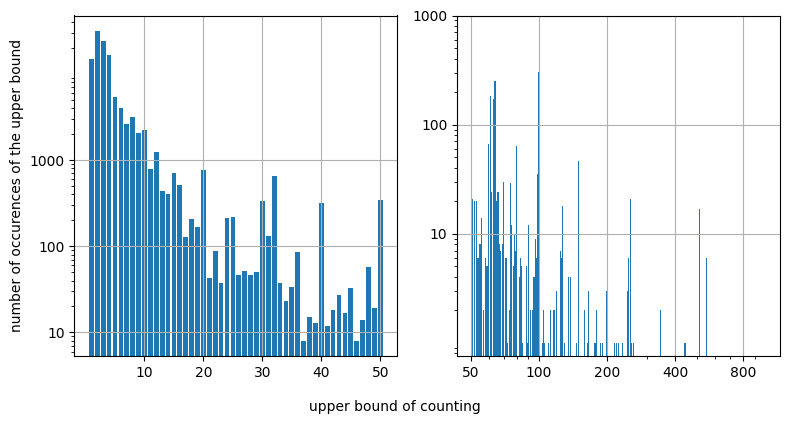
\includegraphics[width=0.9\textwidth]{counting_distribution.png}  
  \caption{Distribution of problem instances w.r.t. counting bounds}  
  \label{fig:count_distri}
\end{figure}

\subsection{Performance evaluation against the other solvers}\label{subsec:overall_eval}

We evaluate the performance of $\ostrichrecl$ against the state-of-the-art string constraint solvers, including CVC5
\cite{cvc5}, Z3seq \cite{z3seq}, Z3str3
\cite{Z3-str3}, Z3str3RE \cite{BD+23}, and OSTRICH
\cite{CHL+19}, on RegCoL, AutomatArk and NestC benchmark suites.
The experiment results can be found in Table~\ref{tab:table_overall_eval}. Note that we take the results of CVC5 as the ground truth\footnote{Initially,  we used the majority vote of the results of the solvers as the ground truth. Nevertheless, on some problem instances, all the results of the three solvers in the Z3 family are wrong (after manual inspection), thus failing this approach on these instances.}, and the results different from the ground truth are classified as \emph{error}. We can see that $\ostrichrecl$ solves almost all instances, except 182 of them, that is, it solves 49,638 instances correctly. The number is 4,547/1,917/13,618/2,764/3,134 more than the number of instances solved by CVC5/Z3str3RE/Z3str3/Z3seq/OSTRICH respectively.
%
Moreover, $\ostrichrecl$ is the second fastest solver, whose average time on each instance is close to the fastest solver Z3str3RE (2.88s versus 1.99s). 

\begin{table}
  \centering\vskip 0pt
    \import{tables}{table_regcol.tex}
    \caption{Overall performance evaluation}
  \label{tab:table_overall_eval}
\end{table}
%To answer \textbf{Q1}, \textbf{$\ostrichrecl$ is the second fastest solver on these benchmark suites, and it solves the most number of instances}.


% \subsection{Evaluation on problem instances with large bounds}\label{subsec:large_bounds_eval}
% We extract \denghang{todo} problem instances with large sum of counting upper bounds (greater than or equal to $50$) from the three benchmark suites.  
% Moreover, in order to test the performance of the solvers on string constraints with large length bounds as well, we increase the length bound to $50$, that is, $|x| > 50$.

% We evaluate the performance of $\ostrichrecl$ on the \denghang{todo} instances. 
% The experiment results can be found in Table~\ref{tab:large-bound}. We can see that $\ostrichrecl$ solves 1,873 instances correctly, which is 947/278/563/637/523 more than those solved by CVC5/Z3str3RE/Z3str3/Z3seq/OSTRICH respectively. Furthermore, $\ostrichrecl$ is 6.79/2.88/2.61/5.27/3.95 times faster than CVC5/Z3str3RE/ Z3str3/Z3seq/OSTRICH respectively. From the results, we can conclude that $\ostrichrecl$ is much more effective and efficient to solve the problem instances with large bounds than the other solvers.  
%To answer \textbf{Q1}, we can see that $\ostrichrecl$ \textbf{is far more efficient than the other solvers on problem instances with large bounds.}

% \begin{table}[H]
%   \import{tables}{table_large_count.tex}
%   \caption{The performance of solvers on instances with large bounds}\label{tab:large-bound}
% \end{table}

\subsection{Evaluation of the technical choices and optimizations in Section~\ref{sec:algorithm}-\ref{sec-opt-sol-gen}}\label{subsec:size_reduction_eval}

At first, we do experiments to evaluate the effectiveness of the automata size-reduction techniques (i.e. Step 2) in Section~\ref{sec:algorithm}. Then we justify our technical choices of reducing the satisfiability problem to that of LIA formulas and resort to the SMT solvers to solve them. Specifically, we compare $\ostrichrecl$ with a variant where the nuXmv model checker like \cite{atva2020} is used to solve the $\cefadec$ problem. 
%
%We practically answer why we choose LIA formula to solve the nonemptiness problem instead of using the nuXmv model checker like \cite{atva2020}. 
We also evaluate the effectiveness of the optimizations in Section~\ref{sec:heuristic}, i.e. the optimizations for the nesting of counting operators as well as the nesting of counting operators and a complement operator. Finally, we evaluate the effectiveness of the optimizations for the model generation in Section~\ref{sec-opt-sol-gen}. 

%Finally, we carry out experiment on the NestC benchmarks to justify the optimizations of Section~\ref{sec:heuristic} for non-register-representable regexes.
%\subsubsection{Empirical justification of the technical choices}
%We also do experiments to evaluate the effectiveness of the automata size-reduction techniques, that is, Step 2 in Section~\ref{subsec:cefadec}. 
%Let us use $\ostrichrecl_{\rm -SIMP}$ to denote $\ostrichrecl$ with the size-reduction techniques removed. 

\paragraph*{Evaluation of the technical choices and optimizations in Section~\ref{sec:algorithm}}
%
We compare $\ostrichrecl$ with its variant  $\ostrichrecl_{\rm +NUXMV}$, which is obtained from $\ostrichrecl$ by using the nuXmv model checker to solve the $\cefadec$ problem. Moreover, we also compare $\ostrichrecl$ with its variant $\ostrichrecl_{\rm -ASR}$, which is obtained from $\ostrichrecl$ by removing the automata size-reduction technique (i.e. Step 2 in Section~\ref{subsec:cefadec}). 

The experiment results can be found in Table~\ref{tab:results_algorithm}. From the results, we can see that $\ostrichrecl$ solves 2,532 more instances and is 2.38 times faster than $\ostrichrecl_{\rm +NUXMV}$. 
Therefore, the technical choice in Section~\ref{sec:algorithm} where LIA formulas are computed and then solved by the SMT solvers is reasonable, since $\ostrichrecl$ with this technical choice is more efficient than $\ostrichrecl_{\rm +NUXMV}$, where nuXmv is used to solve the $\cefadec$ problem. 
%
Moreover, $\ostrichrecl$ solves 1,083 more instances and is 1.65 times faster than $\ostrichrecl_{\rm -ASR}$. 
From the results, we can see that the automata-size reduction technique indeed plays an important role for the performance improvement. 

\begin{table}
  \import{tables}{table_algorithm.tex}
  \caption{Evaluation of the technical choices and optimizations in Section~\ref{sec:algorithm}}\label{tab:results_algorithm}
\end{table}

%\subsubsection{Empirical justification of the optimizations for register-representable regexes}

\zhilin{stopped here}

\paragraph*{Evaluation of the optimizations in Section~\ref{sec:heuristic}}
%
%\subsubsection{Empirical evaluation of the optimizations for non-regesiter-representable regexes} 
We also compare the performance of $\ostrichrecl$ with its variants ${\rm -NEST}$, ${\rm -COMP}$, ${\rm -FIND}$. ${\rm -NEST}$ is obtained from $\ostrichrecl$ by removing the heuristic for nested counting. ${\rm -COMP}$ is obtained by removing the heuristic for complement on counting operators. ${\rm -FIND}$ is obtained by removing the heuristic for finding the accepted word of the automaton.

\begin{table}
  \import{tables}{table_heuristics_complex.tex}
  \caption{Evaluation of the optimizations in Section~\ref{sec:heuristic}}\label{tab:results_heuristic_complex}
\end{table}

The overall experiment results can be found in Table~\ref{tab:results_heuristic}. We can see that $\ostrichrecl$ solves 77/388/349 more instances and is 1.13/1.18/1.24 times faster than ${\rm -NEST}$/${\rm -COMP}$/${\rm -FIND}$ respectively. 

Since the non-register-representable regexes collected from real world are few (5\% of RegCoL and AutomatArk benchmark suites) and simple, there seems no much difference between the performance of $\ostrichrecl$ and its variants ${\rm -NEST}$, ${\rm -COMP}$, ${\rm -FIND}$ in the overall experiment results. Therefore, we consider the NestC benchmark suite, which contains more complex non-register-representable regexes, to justify the optimizations for non-register-representable regexes. The NestC benchmark experiment results is shown in Table~\ref{tab:results_heuristic_complex}. We can see that $\ostrichrecl$ solves 82/339/326 more instances and is 1.02/1.92/1.61 times faster than ${\rm -NEST}$/${\rm -COMP}$/${\rm -FIND}$ respectively. From the results, we can conclude that all the optimizations sharply improve the performance of $\ostrichrecl$ on the non-register-representable regexes.

\paragraph*{Evaluation of the optimizations in Section~\ref{sec-opt-sol-gen}}

Table~\ref{tab:results_model-gen}. 

\begin{table}
  \import{tables}{table_heuristics_model_gen.tex}
  \caption{Evaluation of the optimizations for the model generation in Section~\ref{sec-opt-sol-gen}}\label{tab:results_model-gen}
\end{table}



%To answer \textbf{Q3}, \textbf{our algorithm for solving the nonemptiness problem is much better than the \textsc{nuXmv}-based techniques}.
